% readme.tex -- a short example of how each Stata Journal insert should be
% organized.

\inserttype{article}

\author{Short article author list}{%
	Kerui Du\\
	School of Management\\
	Xiamen University\\
	Xiamen, China\\
	kerrydu@xmu.edu.cn \\
	\\
	
	\and
	Luis Orea \\
	Department of Economics \\
	School of Economics and Business\\
	University of Oviedo \\
	Oviedo, Spain \\
	lorea@uniovi.es \\
	\\
	
	\and
	Inmaculada C. Álvarez \\
	Department of Economics \\
	Universidad Autónoma de Madrid \\
	Madrid, Spain\\
	inmaculada.alvarez@uam.es
  
  
}

\title[Short toc article title]{Fitting spatial stochastic frontier models in Stata}
\maketitle


\begin{abstract}
In this article, we introduce a new command spxtsfa for fitting spatial stochastic frontier models in Stata. Over the last decades, an important theoretical progress of stochastic frontier models is the incorporation of various types of spatial components. Models with the ability to account for spatial dependence and spillovers have been developed for efficiency and productivity analysis, drawing extensive attention from industry and academia. Due to the unavailability of the statistical packages, the empirical applications of the new stochastic frontier models appear to be lagging. The spxtsfa command provides a routine for estimating the spatial stochastic frontier models in the style of \cite{orea2019new} and \cite{galli2022spatial}, enabling users to handle different sources of spatial dependence. In the presented article, we introduce the spatial stochastic frontier models, describe the syntax and options of the new command, and provide several examples to illustrate its usage.
	
	\keywords{stochastic frontier models, SFA, spatial dependence, technical efficiency, spillovers }
\end{abstract}


% discussion of the Stata Journal document class.
%\input sj.tex
% discussion of the Stata Press LaTeX package for Stata output.
%\input stata.tex

\section{Introduction}\label{sec_intro}
%[background]


Producers might fail in optimizing their production activities, causing deviation from the maximum output or the minimum cost. Economic researchers proposed the concept of technical efficiency, which measures how well a producer is utilizing its resources to produce goods or services. A technically efficient organization makes the maximum outputs given the amount of inputs or uses the minimum amount of inputs to produce a given level of output. On the contrary, technically inefficient organization produce fewer outputs given the same inputs or uses more inputs than necessary to produce the same output. Technical efficiency is important because it allows organizations or economies to achieve their goals with the least amount of resources possible, which can lead to cost savings and increased profitability. 

\cite{aignerFormulationEstimationStochastic1977} and \cite{meeusen1977efficiency} introduced stochastic frontier models for evaluating technical efficiency. The essential concept behind these models is to divide the observed output of a production process into two components, namely the "frontier" output, signifying the maximum feasible output, given the inputs utilized in the production process, and the "residual" output, denoting the production process's inefficiency. Following these initial works, stochastic frontier models gained extensive use as a tool for scrutinizing productivity and efficiency. 

Methodologically, econometricians have expanded the horizons of stochastic frontier models in various directions. To name a few, \cite{battese1995model} incorporated the determinants of inefficiency. \cite{wang2003stochastic} developed the stochastic frontier model with scaling properties to capture the shape of the distribution of inefficiency. \cite{greene2005fixed} extended the stochastic models with the random effects and the “true” fixed effects. \cite{belotti2018consistent}, \cite{chen2014consistent}, and \cite{ wang2010estimating} circumvented the "incidental parameters problem" in the fixed effects stochastic frontier model through model transformation. \cite{karakaplan2017handling} developed an endogenous stochastic frontier model to control for the endogeneity in the frontier or inefficiency. 


In recent years, stochastic frontier models have undergone further extension to account for spatial dependence and spatial spillover effects. \cite{glass2016spatial} constructed a spatial Durbin stochastic model considering both global and local spatial dependence. \cite{kutluSpatialStochasticFrontier2020} proposed a spatial stochastic frontier model with endogenous frontier and environmental variables. \cite{glass2016spatial} and \cite{kutluSpatialStochasticFrontier2020} combine the concepts of spatial econometrics and stochastic frontier analysis by including the spatial lag of the dependent variable. On the other hand, \cite{orea2019new} developed a new stochastic frontier model with spatial correlation in both noise and inefficiency terms. \cite{galli2022spatial} integrated the two different modeling ideas to specify four different sources of spatial dependence fully.  


With the increasing demand in the last decades to analyze technical efficiency, Stata provides official commands frontier and xtfrontier for cross-sectional and panel stochastic model estimation, respectively. \cite{belotti2013stochastic} developed sfcross and sfpanel commands accommodating more different distribution assumptions and allowing fixed-effect and random-effect models with the consideration of heteroscedasticity. \cite{karakaplan2017fitting} introduced the sfkk command for estimating endogenous stochastic frontier models. \cite{mustafaugurkarakaplan2018xtsfkk} supplemented the xtsfkk command for fitting the endogenous panel stochastic frontier model. \cite{kumbhakarpractitioner} provides a practitioner’s guide to stochastic frontier analysis with a suite of Stata commands (including sfmodel, sfpan, sf\_fixeff, and sfprim).

In this article, we introduce spxtsfa, a new command for fitting spatial stochastic frontier models in the style of \cite{orea2019new} and \cite{galli2022spatial}. The proposed spxtsfa command not only allows getting more accurate inefficiency scores \citep[see e.g.][]{orea2018spatial} but also examining relevant economic issues that a non-spatial stochastic frontier model tends to overlook. For instance, in microdata applications, the new command can be used to test whether the production/cost function can be viewed as a purely deterministic (engineering) process where the firm controls all the inputs \citep[see e.g.][]{druska2004generalized}. A distinctive feature of the spxtsfa command is that it allows estimating a stochastic frontier model with cross-sectional correlation in the inefficiency term, a specification that is useful in applications where some firms benefit from best practices implemented in adjacent firms due to, for instance, agglomeration economies, knowledge spillovers, technology diffusion or R\&D spillovers. This could especially be the case if (local) firms belong to communitarian networks (e.g. cooperatives) or common technicians (consultants) are advising all local firms. In practice, the proposed spxtsfa command can be useful to capture a kind of behavioral correlation, for instance when firms tend to “keep an eye” on the decisions of other peer firms trying to overcome the limitations caused by the lack of information or they simply emulate each other. It is finally germane to mention that the spxtsfa command also allows capturing cross-sectional effects that might be caused by non-spatial factors (e.g., the regulation environment) if we define appropriately the so-called weight (W) matrix. A proper definition of the W matrix might, for instance, allow us to examine the existence of knowledge spillovers from supplier and user firms. 

As \cite{orea2019new} point out, the proposed spxtsfa command can be implemented using macro-level data (e.g. data of countries, regions or industries) due to the abundant evidence of important feedback processes between neighboring or non-distant regions justify the use of SAR and Durbin frontier functions in macrodata applications. The spatial weight matrix specification commonly adopted in regional economics is based on geographical distance. However, as aforementioned, the weight matrix can be defined using a non-spatial criterion.  In this sense, \cite{liu2023industry} state that the mode of production in the world economy is characterized by the division of global value chains (GVCs) and, hence, the spatial weight matrix should be constructed using the economic distance between industries within/across national economies. In this case, the proposed spxtsfa command can be used to estimate spatial SAR and Durbin frontier functions in order to examine the diffusion of knowledge and technology among the participants in the international production network. It is also makes sense to estimate a stochastic frontier model with cross-sectional correlation in the inefficiency term using macrodata if we change the interpretation of the estimated correlation. In these applications, the spatial correlation in the inefficiency term likely captures barriers and distortions to the efficient allocation of resources across firms that are common to several regions, such as regulation, labor market trends or common institutions \citep[see e.g.][]{orea2023industry}.  


The remainder of this article unfolds as follows: Section 2 provides a brief description of the models in \cite{orea2019new} and \cite{galli2022spatial}; Section 3 explain the syntax and options of spxtsfa; Section 4 and 5 present simulated data examples to illustrate the usage of the command; and section 6 concludes the article.


\section{The model}\label{sec_method}
%[intro]
In this section, we briefly describe the spatial stochastic frontier models developed by \cite{orea2019new} and \cite{galli2022spatial}. The exposition here is only introductory. Please refer to the cited papers for more technical details.  

Based on the transposed version of \cite{wang2010estimating} model, \cite{orea2019new}  proposed a spatial stochastic frontier model which accommodates spatially-correlated inefficiency and noise terms. The model is formulated as in Eqs.\eqref{eq1}-\eqref{eq3}, for $i=1,...,N$ and $t=1,..,T$:

\begin{equation}\label{eq1}
 Y_{it} = X_{it}'\beta + \tilde{v}_{it}-s\tilde{u}_{it}
\end{equation}

\begin{equation}\label{eq2}
	\tilde{v}_{it} =v_{it}+ \gamma W_{i}^{vt}\tilde{v}_{.t} 
\end{equation}

\begin{equation}\label{eq3}
	\tilde{u}_{it} =u_{it}+ \tau W_{i}^{ut}\tilde{u}_{.t} 
\end{equation}

 Eq.\eqref{eq1}  describes the stochastic frontier function where $Y_{it}$ is the dependent variable and $X_{it}$ is a $k \times 1$ vector of variables shaping the frontier; $s=1$ for the production function and  $s=-1$ for the cost function; $\tilde{v}_{it}$ and $\tilde{u}_{it}$ represent  idiosyncratic noise and inefficiency, respectively. In  Eqs.\eqref{eq2} and \eqref{eq3}, $W_{i}^{vt}=(W_{i1}^{vt},...,W_{iN}^{vt})$ and $W_{i}^{vt}=(W_{i1}^{vt},...,W_{iN}^{vt})$ are two known $1 \times N$ cross-sectional weight vectors  depicting the structure of the  cross-sectional relationship for idiosyncratic noise and inefficiency terms, respectively; $\tilde{v}_{.t}=(\tilde{v}_{1t},...,\tilde{v}_{Nt})' $ and $\tilde{u}_{.t}=(\tilde{u}_{1t},...,\tilde{u}_{Nt})'$; $v_{it}$  is a random variable following the distribution $N(0,\sigma_v^2)$ and $u_{it}=h(Z_{it}'\delta)u_t^*$. $h(Z_{it}'\delta)$ is the scaling function where $Z_{it}$ is a $l \times 1$ vector of variables affecting individuals' inefficiency  and $u_t^*$ is a non-negative random variable following the distribution $N^+(0,\sigma_{u}^2)$.  Using matrix notation, we can rewrite Eqs.\eqref{eq2} and \eqref{eq3} as
 
 \begin{equation}\label{eq2b}
 	\tilde{v}_{.t} =(I_N-\gamma W^{vt})^{-1}v_{.t} 
 \end{equation}
 
 \begin{equation}\label{eq3b}
 		\tilde{u}_{.t} =(I_N-\tau W^{ut})^{-1}h(Z_{.t}\delta)u_t^* = \tilde{h}_{.t}u_t^*
 \end{equation}
 where $Z_{.t}=(Z_{1t},...,Z_{Nt})'$;$\tilde{h}_{.t}=(I_N-\tau W^{ut})^{-1}h(Z_{.t}\delta)$.
 
  The above model captures the spatial correlation of  the random error and inefficiency terms with the spatial autoregressive (SAR) process \footnote{\cite{orea2019new} also considered a specification of the spatial moving average process.}.  Referring to \cite{wang2010estimating}, we can obtain the following log-likelihood function for each period $t$:
  \begin{equation}\label{eq5}
 	\begin{aligned}
 		\ln L_{t}= & -\frac{N}{2} \ln (2 \pi)-\frac{1}{2} \ln |\Pi|-\frac{1}{2} \tilde{\varepsilon}_{.t} \Pi^{-1} \tilde{\varepsilon}_{.t} \\
 		& +\frac{1}{2}\left(\frac{\mu_{*}^{2}}{\sigma_{*}^{2}}\right)+\ln \left[\sigma_{*} \Phi\left(\frac{\mu_{*}}{\sigma_{*}}\right)\right]-\ln \left(\frac{1}{2}\sigma_{u} \right)
 	\end{aligned}
 \end{equation}
where $\Pi=\sigma_v^2(I_N-\rho W^{yt})^{-1}[(I_N-\rho W^{yt})^{-1}]'$; $ \tilde{\varepsilon}_{.t} = ( \tilde{\varepsilon}_{1t},..., \tilde{\varepsilon}_{Nt})', \tilde{\varepsilon}_{it}=s(Y_{it}-X_{it}' \beta)$, and 
\begin{equation}
	\mu_*  =\frac{-\tilde{\varepsilon}_{.t}^{\prime} \Pi^{-1} \tilde{h}_{.t}}{\tilde{h}_{.t}' \Pi^{-1} \tilde{h}_{.t}+1 / \sigma_u^2}
\end{equation}
\begin{equation}
	\sigma_*^2  =\frac{1}{\tilde{h}_{.t}^{\prime} \Pi^{-1} \tilde{h}_{.t}+1 / \sigma_u^2}
\end{equation}

 
\cite{galli2022spatial} further incorporated the spatial lags of the dependent variable and the input variables into \cite{orea2019new} model, which additionally measures global and local spatial spillovers affecting the frontier function.  The model is expressed as
\begin{equation}\label{gallimodel}
	Y_{it} = \rho W_{i}^{yt}Y_{.t}+X_{it}'\beta+ W_{i}^{xt}X_{.t} \theta + \tilde{v}_{it}+s\tilde{u}_{it}
\end{equation}
where $W_{i}^{yt}=(W_{i1}^{yt},...,W_{iN}^{yt})$ and $W_{i}^{xt}=(W_{i1}^{xt},...,W_{iN}^{xt})$ are two known $1 \times N$ cross-sectional weight vectors \footnote{We index $W_{i}^{yt}$, $W_{i}^{xt}$, $W_{i}^{ut}$, and $W_{i}^{vt}$ with superscript $yt$, $xt$, $ut$, and $vt$, respectively. This indicates the spatial weight matrix can be time-varying and different across various spatial components}; $Y_{.t} = (Y_{1t},..., Y_{Nt})'$; $X_{.t} = (X_{1t},..., X_{Nt})'$.  This model gives rise to the following log-likelihood function for each period $t$: 

  \begin{equation}\label{gallilik}
	\begin{aligned}
		\ln L_{t}= & ln|I_N - \rho W^{yt}|-\frac{N}{2} \ln (2 \pi)-\frac{1}{2} \ln |\Pi|-\frac{1}{2} \tilde{\varepsilon}_{.t} \Pi^{-1} \tilde{\varepsilon}_{.t} \\
		& +\frac{1}{2}\left(\frac{\mu_{*}^{2}}{\sigma_{*}^{2}}\right)+\ln \left[\sigma_{*} \Phi\left(\frac{\mu_{*}}{\sigma_{*}}\right)\right]-\ln \left(\frac{1}{2}\sigma_{u} \right)
	\end{aligned}
\end{equation}
where $ \tilde{\varepsilon}_{.t} = ( \tilde{\varepsilon}_{1t},..., \tilde{\varepsilon}_{Nt})', \tilde{\varepsilon}_{it}=s(Y_{it}-X_{it}' \beta - \rho W_{i}^{yt}Y_{.t} -W_{i}^{xt}X_{.t} \theta)$. 

Summing the time-specific log-likelihood  functions over all periods yields the overall likelihood function for the whole sample, i.e., $lnL=\sum_{t=1}^TlnL_{t}$. Then, numerically maximize the overall log-likelihood function to obtain consistent estimates of the parameters in the above models.  Specifically, we use Stata {\tt ml model} routine with the {\tt method-d0} evaluator to program the {\tt spxtsfa} command. Following \cite{gude2018heterogeneous}, we parameterize $\rho$, $\gamma$, and $\tau$ as Eq.\eqref{para} to ensure the standard regularity condition for the spatial autoregressive models.
\begin{equation}\label{para}
\begin{aligned}
	& \eta=\left(\frac{1}{r_{\text {min }}}\right)(1-p)+\left(\frac{1}{r_{\max }}\right) p \\
	& 0 \leq p=\frac{\exp \left(\delta_0\right)}{1+\exp \left(\delta_0\right)} \leq 1
\end{aligned}
\end{equation}
where $\eta$ stands for one of $\rho$, $\gamma$, and $\tau$;  $r_{\text {min }}$ and $r_{\text {max}}$ are respectively the minimum and maximum eigenvalues of the corresponding spatial weight matrix. 

In summary, \cite{galli2022spatial} provided a fully comprehensive specification of four different types of spatial dependence: global spillovers of dependent variable $Y_{it}$, local spillovers of input variables $X_{it}$, cross-sectional correlation of idiosyncratic noise  $v_{it}$ and inefficiency $u_{it}$. We term this full model "$yxuv$-SAR". Some restrictions can be imposed on the specific parameters to generate the following  models (summarized in Table \ref{Tab01}), which can be estimated by the {\tt spxtsfa} command.


% Please add the following required packages to your document preamble:
% \usepackage{booktabs}
\begin{table}[htbp]
	%\scriptsize
	
	\centering
	
	\caption{Specific  models with restricted parameters}
	
	\label{Tab01}
	\begin{tabular}{@{}llllllllllll@{}}
		\toprule
		 & $yuv$ & $xuv$ & $yv$ & $yu$ & $y$ & $xuv$ & $xv$ & $xu$ & $uv$ & $u$ & $v$  \\ \midrule
		$\rho$   &     & 0   &    &    &   & 0   & 0  & 0  & 0  & 0 & 0 \\
		$\theta$ & 0   &     & 0  & 0  & 0 &     &    &    & 0  & 0 & 0 \\
		$\gamma$ &     &     &    & 0  & 0 &     &    & 0  &    & 0 &   \\
		$\tau$   &     &     & 0  &    & 0 &     & 0  &    &    &   & 0 \\ \bottomrule
	\end{tabular}
\end{table}



\endinput

% discussion of the Stata Press LaTeX package for Stata output.

\section{The xtsfsp command}
\vspace{5pt}
\stcmd{xtsfsp} estimates spatial stochastic frontier models in the style of \cite{orea2019new} and \cite{galli2022spatial}.

\subsection{Syntax}
\vspace{5pt}
Estimation syntax

\begin{stsyntax}
	xtsfsp\
    \depvar\
    \optindepvars,\
    uhet(\varlist \optional{,noconstant})		
	\optional{vhet(\varlist \optional{,noconstant})
		cost
		noconstant
		wy({\it wyspec})
		wx({\it wxspec})
		wu({\it wuspec})
		wv({\it wvspec})
		normalize({\it norm\_method})
		wxvars(\varlist)
		\underbar{init}ial({\it matname})
		mlmodel({\it model\_options})
		mlsearch({\it search\_options})
		mlplot
		mlmax({\it maximize\_options})
		nolog
		mldisplay({\it display\_options})
		level(\num)
		te(\newvarname)
		genwxvars
		delmissing
		constraints({\it constraints})
	}
\end{stsyntax}



\noindent Version syntax

\begin{stsyntax}
	xtsfsp\
	, version
\end{stsyntax}


\noindent Replay syntax

\begin{stsyntax}
	xtsfsp\
	\optional{, level(\num) }
\end{stsyntax}

\subsection{Options}
\vspace{5pt}
\hangpara
{\tt uhet(\varlist [,noconstant])} specifies explanatory variables for scaling  function depending on a linear combination of \varlist. Use nonconstant to suppresses constant term.

\hangpara
{\tt vhet(\varlist [,noconstant])} specifies explanatory variables for idiosyncratic error variance function depending on a linear combination of \varlist. Use nonconstant to suppresses constant term.

\hangpara
{\tt noconstant} suppresses constant term.

\hangpara
{\tt cost} specifies the frontier as a cost function. By default, the production function is assumed.

\hangpara
{\tt wy({\it wyspec})} specifies the spatial weight matrix for the dependent variable. The expression is wy($W_1$ $ [W_2 ... W_T]$ [,{\it mata array}]).  By default, the weight matrices are \stcmd{spmatrix} objects created by Stata official command \stcmd{spmatrix}. mata declares weight matrices are Mata matrices. If one weight matrix is specified, it assumes a time-constant weight matrix. For time-varying cases, $T$ weight matrices should be specified in time order. Alternatively, using array to declare weight matrices are stored in an array.  If only one matrix is stored in the specified array, the time-constant weight matrix is assumed.  Otherwise, the keys of the array specify time information, and the values store time-specific weight matrices.

\hangpara
{\tt wx({\it wxspec})} specifies the spatial weight matrix for spatial During terms. The expression is the same as {\tt wy({\it wyspec})}.

\hangpara
{\tt wu({\it wuspec})} specifies spatial weight matrix for spatial spillover of inefficiency . The expression is the same as {\tt wy({\it wyspec})}.

\hangpara
{\tt wv({\it wvspec})} specifies spatial weight matrix for spatial dependence of random error. The expression is the same as {\tt wy({\it wyspec})}.

\hangpara
{\tt normalize({\it norm\_method})} specifies  one of the four available normalization techniques: row, col, minmax, and spectral.

\hangpara
{\tt wxvars(\varlist)} specifies variables for spatial Durbin terms.


\hangpara
{\tt \underbar{init}ial({\it matname})} specifies  the initial values of the estimated parameters with matrix {\it matname}.

\hangpara
{\tt mlmodel({\it model\_options})} specifies the  {\tt ml model} options.

\hangpara
{\tt mlsearch({\it search\_options})} specifies the  {\tt ml search} options.

\hangpara
{\tt mlplot} specifies using  {\tt ml plot} to search better initial values of spatial dependence parameters.

\hangpara
{\tt mlmax({\it maximize\_options})} specifies the  {\tt ml maximize} options.

\hangpara
{\tt nolog} suppresses the display of the criterion function iteration log.

\hangpara
{\tt mldisplay({\it display\_options})} specifies the  {\tt ml display} options.

\hangpara
{\tt level(\num)} sets confidence level; default is level(95).

\hangpara
{\tt te({\it newvarname})} specifies a new variable name to store the estimates of technical efficiency.

\hangpara
{\tt genwxvars} generates the spatial Durbin terms. It is activated only when {\tt wxvars(\varlist)} is specified.

\hangpara
{\tt delmissing} allows estimation  when missing values are present by  removing the corresponding units from spatial matrix. 

\hangpara
{\tt constraints(\it constraints)}  specifies linear constraints for the estimated model. 


\subsection{Dependency of xtsfsp}
\vspace{5pt}
\stcmd{xtsfsp} depends on the \stcmd{moremata} package contributed by  \cite{BenJann}. If not already installed, you can install it by typing {\tt ssc install moremata}. 


%\section{Examples with simulated data}\label{sec_example}
\section{Examples}\label{sec_example}
\vspace{5pt}

The \stcmd{xtsfsp} command described above offers great flexibility, allowing for various specifications of spatial dependence. Specifically, it enables the specification of different combinations of spatial components, with the option to have different and time-varying spatial weight matrices. Furthermore, it allows for the specification of conditional heteroscedasticity of random errors. In this section, we present four examples that demonstrate the usage of the \stcmd{xtsfsp} command. To run the following examples, some Community-contributed packages \stcmd{tictoc} \citep{tictoc}, \stcmd{translog} \citep{translog}, \stcmd{graph2tex} \citep{graph2tex} need to be installed in advance \footnote{We run the codes with Stata 18 MP (16 Cores) in a Mac mini (M2 Chip, 16G RAM).}. 

\subsection{yxuv-SAR model with time-invariant spatial weight matrices}
\vspace{5pt}
Referring to  \cite{galli2022spatial}, we first consider the yxuv-SAR model specified by the following data-generating process (DGP 1) with $i=1,...,300$ and $t=1,..,20$,

\begin{equation}\label{dgp1}
	y_{it} = 0.3W_{i}y_{.t}+2x_{it}+ 0.5W_{i}x_{.t}  + \tilde{v}_{it}-\tilde{u}_{it}
\end{equation}
where $\tilde{v}_{it}$ and $\tilde{u}_{it}$ are defined as in Eqs.\eqref{eq2} and \eqref{eq3} with $\gamma=0.3$, $\tau=0.3$, $Z_{it}=(z_{it},1)'$,$\delta=(2, ln(0.2))'$, $D_{it}=1$ and $\eta = ln(0.2)$. All the spatial matrices for the four spatial components are the same and time-invariant, created from a binary contiguity spatial weight matrix. We generate the exogenous variables $X_{it}$ and $z_{it}$ from the standard normal distribution, respectively. With the sample generated by DGP 1, we can fit the model into the following syntax.

\begin{stlog}
	. use xtsfsp_ex1.dta
{\smallskip}
. xtset id t 
{\smallskip}
Panel variable: id (strongly balanced)
 Time variable: t, 1 to 20
         Delta: 1 unit
{\smallskip}
. * importing spatial weight matrix from xtsfsp_wmat1.mmat
. mata mata matuse xtsfsp_w1.mmat,replace
(loading w1[300,300])
{\smallskip}
. * fitting the model
. tic
Timer is turned on!
{\smallskip}
. xtsfsp y x, uhet(z) wu(w1,mata) wy(w1,mata) wv(w1,mata) ///
>             wx(w1,mata) wxvars(x) te(te) nolog
{\smallskip}
Spatial frontier model(yxuv-SAR)                     Number of obs =     6,000
                                                     Wald chi2(2)  = 113733.00
Log likelihood = -3953.6034                          Prob > chi2   =    0.0000
{\smallskip}
\HLI{13}{\TOPT}\HLI{64}
           y {\VBAR} Coefficient  Std. err.      z    P>|z|     [95\% conf. interval]
\HLI{13}{\PLUS}\HLI{64}
frontier     {\VBAR}
           x {\VBAR}   2.006736   .0082953   241.91   0.000     1.990477    2.022994
         W_x {\VBAR}   .5457545   .0709898     7.69   0.000     .4066171    .6848919
       _cons {\VBAR}   1.008833   .0460347    21.91   0.000     .9186065    1.099059
\HLI{13}{\PLUS}\HLI{64}
    /lnsigv2 {\VBAR}  -1.566886   .0184019   -85.15   0.000    -1.602953   -1.530819
\HLI{13}{\PLUS}\HLI{64}
uhet         {\VBAR}
           z {\VBAR}   .9858524   .0385881    25.55   0.000      .910221    1.061484
       _cons {\VBAR}  -1.533232   .3361919    -4.56   0.000    -2.192156   -.8743081
\HLI{13}{\PLUS}\HLI{64}
Wy           {\VBAR}
       _cons {\VBAR}     .57773    .062202     9.29   0.000     .4558163    .6996436
\HLI{13}{\PLUS}\HLI{64}
Wv           {\VBAR}
       _cons {\VBAR}   .6066382   .0743834     8.16   0.000     .4608494     .752427
\HLI{13}{\PLUS}\HLI{64}
Wu           {\VBAR}
       _cons {\VBAR}   .6584973   .0938095     7.02   0.000      .474634    .8423606
\HLI{13}{\PLUS}\HLI{64}
         rho {\VBAR}   .2810617   .0286408     9.81   0.000     .2240201    .3361839
       gamma {\VBAR}   .2943177    .033966     8.67   0.000     .2264087    .3593786
         tau {\VBAR}   .3178137    .042162     7.54   0.000     .2329366    .3978845
\HLI{13}{\BOTT}\HLI{64}
Note: Wy:_cons, Wv:_cons and Wu:_cons are the transformed parameters;
      rho, gamma and tau are their origin metrics in spatial components, respectiv
> ely.
      W_(x) represent Spatial Durbin terms W(x)
{\smallskip}
. toc
Elapsed time: 252.347 sec
             =4 min \& 12.347 sec
{\smallskip}

\end{stlog}

The output shows that the command fits six equations with the {\tt ml model}. The frontier equation has three explanatory variables $x_{it}$, $W_ix_{.t}$ and constant. The scaling function uhet() has two explanatory variables $Z_{it}$ and constant.  The equation  /lnsigv2 is constructed for the variance parameter  $\sigma_v^2$ which is transformed by the function $exp(\cdot)$. Three equations (Wy, Wu, and Wv) handle the spatial dependence parameters $\rho$, $\tau$, and $\gamma$, which are parameterized as Eq.\eqref{para}. We directly include the spatial Durbin term $W_ix_{.t}$ in the frontier equation  (represented by W\_x) such that we do not need to fit a separate equation.  The bottom of the table reports the transformed parameters in the original metric.

\subsection{xuv-SAR model with different spatial weight matrices}
\vspace{5pt}
We consider a restricted model xuv-SAR with different spatial weight matrices, one of which is time-varying, whilst the others are time-constant.  The model is described as DGP 2:
\begin{equation}\label{dgp2}
	y_{it} = 1+2x_{it}+ 0.5W_{i}^{xt}x_{it} + \tilde{v}_{it}+\tilde{u}_{it}, i=1,..,300; t=1,..,10
\end{equation}
where the other parameters are set the same as in DGP 1 except for $W_{i}^{ut}=W_{i}^u$, $W_{i}^{vt}=W_{i}^v$, $\delta = (4,ln(0.2))'$, and $W_{i}^{xt}$ is time-varying.  Different from DGP 1, which sets the production function frontier, DGP 2 specifies a cost function. The estimation of the model is shown as follows.

\begin{stlog}
	. * importing spatial weight matrices from xtsfsp_w2.mmat
. mata mata matuse xtsfsp_w2.mmat,replace
(loading w1[300,300], w10[300,300], w2[300,300], w3[300,300], w4[300,300], w5[300,300], w6[300,300],
 w7[300,300], w8[300,300], w9[300,300])
{\smallskip}
. local w w1 w2 w3 w4 w5 w6 w7 w8 w9 w10
{\smallskip}
. use xtsfsp_ex2.dta
{\smallskip}
. xtset id t 
{\smallskip}
Panel variable: id (strongly balanced)
 Time variable: t, 1 to 10
         Delta: 1 unit
{\smallskip}
. * initial values for estimated parameters
. mat b=(2,0.5,1,-1.5,4,-1.5,0.6,0.6)
{\smallskip}
. * fitting the model
. xtsfsp y x, cost uhet(z) wu(w2,mata) wv(w1,mata) wxvars(x) wx(`w',mata) init(b) genwxvars nolog
{\smallskip}
Spatial frontier model(xuv-SAR)                       Number of obs =    3,000
                                                      Wald chi2(2)  = 57442.57
Log likelihood = -1911.966                            Prob > chi2   =   0.0000
{\smallskip}
\HLI{13}{\TOPT}\HLI{64}
           y {\VBAR} Coefficient  Std. err.      z    P>|z|     [95\% conf. interval]
\HLI{13}{\PLUS}\HLI{64}
frontier     {\VBAR}
           x {\VBAR}   1.995755   .0083855   238.00   0.000      1.97932     2.01219
         W_x {\VBAR}   .5069275   .0221351    22.90   0.000     .4635435    .5503115
       _cons {\VBAR}   .9917396   .0127293    77.91   0.000     .9667906    1.016689
\HLI{13}{\PLUS}\HLI{64}
    /lnsigv2 {\VBAR}  -1.614693   .0260257   -62.04   0.000    -1.665702   -1.563683
\HLI{13}{\PLUS}\HLI{64}
uhet         {\VBAR}
           z {\VBAR}   3.999532    .002155  1855.94   0.000     3.995308    4.003755
       _cons {\VBAR}   -1.69907   .4472607    -3.80   0.000    -2.575685   -.8224549
\HLI{13}{\PLUS}\HLI{64}
Wv           {\VBAR}
       _cons {\VBAR}   .5877877   .0584046    10.06   0.000     .4733168    .7022585
\HLI{13}{\PLUS}\HLI{64}
Wu           {\VBAR}
       _cons {\VBAR}   .6214134   .0008532   728.34   0.000     .6197412    .6230857
\HLI{13}{\PLUS}\HLI{64}
         tau {\VBAR}   .3010498   .0003879   776.13   0.000     .3002894    .3018098
       gamma {\VBAR}   .2856862   .0268157    10.65   0.000     .2323138    .3373429
\HLI{13}{\BOTT}\HLI{64}
Note: Wv:_cons and Wu:_cons are the transformed parameters;
      gamma and tau are their origin metrics in spatial components, repsectively.
      W_(x) represent Spatial Durbin terms W(x)

\end{stlog}

In the second example, we use a {\tt cost} option to specify the type of frontier. The matrix {\tt b} is utilized as the initial value for maximum likelihood estimation. The likelihood function of spatial stochastic frontier models is intricate and typically challenging when trying to obtain optimal global solutions. Therefore, having good initial values would be beneficial for fitting spatial stochastic models. In order to acquire initial values for spatially-correlated parameters, practitioners can start by fitting non-spatial stochastic models using the \stcmd{frontier} and \stcmd{sfpanel} commands. This way,  the initial values of the parameters involved in the frontier and the scaling function are obtained. Subsequently, the {\tt mlplot} option can be employed to search for better initial values.

To demonstrate the usage of the \textit{delmissing} option, two observations of $y_{it}$ are replaced with missing values, and the aforementioned codes are re-run, resulting in the error message "\textit{missing values found. use delmissing to remove the units from the spmatrix}". The inclusion of the \textit{delmissing} option addresses this issue, and the generated variable \_\_e\_sample\_\_ records the regression sample. The execution time of this example is relatively long, exceeding 17 minutes. This can be attributed to the presence of missing values, which leads to data imbalance and necessitates the computation of time-varying spatial weight matrices due to changing dimensions over time. Equations (4)-(8) involve solving the inverses of three $N \times N$($N \in \{299,300\}$) matrices, and considering the time-varying nature of these matrices, their computation needs to be performed $T$ times in each step for optimizing likelihood functions. Consequently, this particular example takes nearly eight times longer than the previous one.
 
 \begin{stlog}
 	. * replace some observations of y to be missing
. replace y=. if _n==1 | _n==100
(2 real changes made, 2 to missing)
{\smallskip}
. local w w1 w2 w3 w4 w5 w6 w7 w8 w9 w10
{\smallskip}
. * estimation is aborted
. cap noi xtsfsp y x, cost uhet(z) wu(w2,mata) wv(w1,mata) ///
>                     wxvars(x) wx(`w',mata) init(b) nolog
missing values found. use delmissing to remove the units from the spmatrix
invalid syntax
{\smallskip}

 	. * re-estimation with delmissing option 
. local w w1 w2 w3 w4 w5 w6 w7 w8 w9 w10
{\smallskip}
. cap noi xtsfsp y x, cost uhet(z) wu(w2,mata) wv(w1,mata) wxvars(x) wx(`w',mata) init(b) delmissing nolog
missing values found. The corresponding units are deleted from the spmatrix
{\smallskip}
Spatial frontier model(xuv-SAR)                       Number of obs =    2,998
                                                      Wald chi2(2)  = 57433.89
Log likelihood = -1909.3843                           Prob > chi2   =   0.0000
{\smallskip}
\HLI{13}{\TOPT}\HLI{64}
           y {\VBAR} Coefficient  Std. err.      z    P>|z|     [95\% conf. interval]
\HLI{13}{\PLUS}\HLI{64}
frontier     {\VBAR}
           x {\VBAR}   1.996019    .008386   238.02   0.000     1.979583    2.012455
         W_x {\VBAR}   .5065641   .0221295    22.89   0.000     .4631912    .5499371
       _cons {\VBAR}   .9914628    .012715    77.98   0.000     .9665418    1.016384
\HLI{13}{\PLUS}\HLI{64}
    /lnsigv2 {\VBAR}  -1.615516   .0260341   -62.05   0.000    -1.666542    -1.56449
\HLI{13}{\PLUS}\HLI{64}
uhet         {\VBAR}
           z {\VBAR}   3.999476   .0021537  1857.01   0.000     3.995254    4.003697
       _cons {\VBAR}  -1.698894   .4472168    -3.80   0.000    -2.575423   -.8223653
\HLI{13}{\PLUS}\HLI{64}
Wv           {\VBAR}
       _cons {\VBAR}   .5864895   .0584501    10.03   0.000     .4719295    .7010496
\HLI{13}{\PLUS}\HLI{64}
Wu           {\VBAR}
       _cons {\VBAR}   .6214135   .0008525   728.95   0.000     .6197427    .6230843
\HLI{13}{\PLUS}\HLI{64}
         tau {\VBAR}   .3010498   .0003876   776.78   0.000       .30029    .3018092
       gamma {\VBAR}     .28509   .0268466    10.62   0.000     .2316575    .3368072
\HLI{13}{\BOTT}\HLI{64}
Note: Wv:_cons and Wu:_cons are the transformed parameters;
      gamma and tau are their origin metrics in spatial components, repsectively.
      W_(x) represent Spatial Durbin terms W(x)
      Missing values found
      The regression sample recorded by variable __e_sample__

 \end{stlog}
 
 \subsection{uv-SAR model with conditional heteroscedasticity of random errors }
 \vspace{5pt}
We set up a restricted model uv-SAR with time-varying spatial weight matrices and conditional heteroscedasticity of random errors. The DGP 3 is described as
 
 \begin{equation}\label{dgp3}
 	 \begin{aligned}
 		& y_{it} = 1+2x_{it} + \tilde{v}_{it}-\tilde{u}_{it}, i=1,..,300; t=1,..,10  \\
 		& \sigma_{v,it}^2 = exp(1+d_{it})  \\
 		&  h(Z_{it}'\delta) = \sqrt{exp(1+z_{it})}
 	\end{aligned}
 \end{equation}
 where the other parameters are set the same as in DGP 1 except for $W_{i}^{ut}=W_{i}^{vt}=W_{i}^t$. The following syntax estimates the model alongside the results. The computation burden in this example exceeds 11 minutes, primarily attributed to the time-varying configuration of the spatial weight matrices.
 
 \begin{stlog}
 	. * importing spatial weight matrices from xtsfsp_w3.mmat
. mata mata matuse xtsfsp_w3,replace
(loading w1[300,300], w10[300,300], w2[300,300], w3[300,300], w4[300,300], w5[300,300], w6[300,300], w7[300,300], w8[300,300], w9[300,300])
{\smallskip}
. local w w1 w2 w3 w4 w5 w6 w7 w8 w9 w10
{\smallskip}
. use xtsfsp_ex3.dta
{\smallskip}
. xtset id t
{\smallskip}
Panel variable: id (strongly balanced)
 Time variable: t, 1 to 10
         Delta: 1 unit
{\smallskip}
. xtsfsp y x, wu(`w',mata) wv(`w',mata) uhet(z) vhet(d) nolog
{\smallskip}
Spatial frontier model(uv-SAR)                         Number of obs =   3,000
                                                       Wald chi2(1)  = 7472.38
Log likelihood = -5803.0516                            Prob > chi2   =  0.0000
{\smallskip}
\HLI{13}{\TOPT}\HLI{64}
           y {\VBAR} Coefficient  Std. err.      z    P>|z|     [95\% conf. interval]
\HLI{13}{\PLUS}\HLI{64}
frontier     {\VBAR}
           x {\VBAR}   1.988108   .0229991    86.44   0.000     1.943031    2.033185
       _cons {\VBAR}   .8997916   .0737763    12.20   0.000     .7551927    1.044391
\HLI{13}{\PLUS}\HLI{64}
lnsigv2      {\VBAR}
           d {\VBAR}   .9897965   .0259185    38.19   0.000     .9389972    1.040596
       _cons {\VBAR}   .9950927   .0259519    38.34   0.000      .944228    1.045957
\HLI{13}{\PLUS}\HLI{64}
uhet         {\VBAR}
           z {\VBAR}   1.019351   .0458701    22.22   0.000     .9294473    1.109255
       _cons {\VBAR}   1.122574   .4629594     2.42   0.015     .2151904    2.029958
\HLI{13}{\PLUS}\HLI{64}
Wv           {\VBAR}
       _cons {\VBAR}   .6171649   .0431991    14.29   0.000     .5324961    .7018337
\HLI{13}{\PLUS}\HLI{64}
Wu           {\VBAR}
       _cons {\VBAR}   .6471479   .0703691     9.20   0.000      .509227    .7850688
\HLI{13}{\PLUS}\HLI{64}
         tau {\VBAR}    .299117   .0196647    15.21   0.000     .2601042    .3371547
       gamma {\VBAR}   .3127036   .0317402     9.85   0.000     .2492256    .3735057
\HLI{13}{\BOTT}\HLI{64}
Note: Wv:_cons and Wu:_cons are the transformed parameters
      gamma and tau are their origin metrics in spatial components, repsectively.

 \end{stlog}
 
\subsection{Example with real data} 
\vspace{5pt}
We use the real data to exemplify how to conduct the empirical studies with the models and the command  described above.The raw data on the provinces of China, including GDP (denoted as $Y$), investment, labor force (denoted as $L$), the ratio of government expenditure to GDP (denoted as fiscal), the ratio of FDI to GDP (denoted as $fdi$), and trade as a percentage of GDP (denoted as $trade$), is collected from the CSMAR database. All nominal variables are adjusted to constant prices in 1997.  The capital stocks for the provinces are estimated using the perpetual inventory method. The production function is approximated by the translog function, and the inefficiency term's scaling function is assumed to be determined by the ratio of government expenditure to GDP, the ratio of FDI to GDP, and trade as a percentage of GDP. 

 \begin{stlog}
	. * Translate shapefile to Stata format
. cap spshape2dta province
{\smallskip}
. 
. use province 
{\smallskip}
. drop if _ID == 26 | _ID>31
(4 observations deleted)
{\smallskip}
. spset 
{\smallskip}
      Sp dataset: province.dta
Linked shapefile: province_shp.dta
            Data: Cross sectional
 Spatial-unit ID: _ID
     Coordinates: _CX, _CY (planar)
{\smallskip}
. * Create spatial contiguity matrix
. spmatrix create contiguity w_con, normalize(none) 
  weighting matrix in w_con contains 1 island
{\smallskip}
. * Obtain spatial matrix as Mata matrix wm from w_con 
. spmatrix matafromsp wm id = w_con
{\smallskip}
. * Match the iland (_ID = 21) with the nearest province(_ID =19)
. mata: wm[19,21]=1
{\smallskip}
. mata: wm[21,19]=1
{\smallskip}
. * Create spmatrix w_con from Mata matrix wm and rwo-normalized the matrix 
. spmatrix spfrommata w_con= wm id, normalize(row) replace
{\smallskip}
. * Obtain the new spatial matrix as Mata matrix wm from w_con 
. spmatrix matafromsp wm id = w_con
{\smallskip}
. 
. use chnempirical.dta,clear
{\smallskip}
. * Generate varables for the translog function
. qui translog Y K L , time(year) norm 
{\smallskip}
. global x  lnK lnL _t lnK_lnL _t_lnK _t_lnL _t_2 lnK_2 lnL_2
{\smallskip}
. global z fiscal trade fdi
{\smallskip}
. * Fit the model with frontier command
. frontier lnY \$x,uhet(\$z) nolog
{\smallskip}
Stoc. frontier normal/half-normal model               Number of obs =      630
                                                      Wald chi2(9)  = 33273.49
Log likelihood = 307.21728                            Prob > chi2   =   0.0000
{\smallskip}
\HLI{13}{\TOPT}\HLI{64}
         lnY {\VBAR} Coefficient  Std. err.      z    P>|z|     [95\% conf. interval]
\HLI{13}{\PLUS}\HLI{64}
lnY          {\VBAR}
         lnK {\VBAR}   .7939407    .020148    39.41   0.000     .7544513      .83343
         lnL {\VBAR}   .2423919   .0152754    15.87   0.000     .2124527    .2723312
          _t {\VBAR}  -.0159651   .0029995    -5.32   0.000     -.021844   -.0100862
     lnK_lnL {\VBAR}  -.0239117   .0463983    -0.52   0.606    -.1148507    .0670274
      _t_lnK {\VBAR}   .0385162   .0100006     3.85   0.000     .0189153     .058117
      _t_lnL {\VBAR}  -.0212483   .0070556    -3.01   0.003     -.035077   -.0074197
        _t_2 {\VBAR}  -.0064186   .0009174    -7.00   0.000    -.0082166   -.0046206
       lnK_2 {\VBAR}  -.0151869   .0327529    -0.46   0.643    -.0793815    .0490077
       lnL_2 {\VBAR}  -.0604274    .031823    -1.90   0.058    -.1227993    .0019444
       _cons {\VBAR}   .3105853   .0138557    22.42   0.000     .2834287    .3377419
\HLI{13}{\PLUS}\HLI{64}
lnsig2v      {\VBAR}
       _cons {\VBAR}  -4.491706   .0912372   -49.23   0.000    -4.670528   -4.312885
\HLI{13}{\PLUS}\HLI{64}
lnsig2u      {\VBAR}
      fiscal {\VBAR}   .0724787   .0116298     6.23   0.000     .0496848    .0952726
       trade {\VBAR}  -.0790757   .0165127    -4.79   0.000      -.11144   -.0467115
         fdi {\VBAR}  -.0262741    .006819    -3.85   0.000    -.0396391   -.0129091
       _cons {\VBAR}  -2.964112   .3476526    -8.53   0.000    -3.645499   -2.282726
\HLI{13}{\PLUS}\HLI{64}
     sigma_v {\VBAR}   .1058372   .0048281                      .0967849    .1157361
\HLI{13}{\BOTT}\HLI{64}
{\smallskip}
. * Predict the inefficiency term and efficiency scores
. predict double uhat, u
{\smallskip}
. generate double te0 = exp(-uhat) 
{\smallskip}
. * Store the estimated parameters
. mat b0=e(b)
{\smallskip}
. 
. * Fit the model with xtsfsp command
. xtset _ID year
{\smallskip}
Panel variable: _ID (strongly balanced)
 Time variable: year, 1997 to 2017
         Delta: 1 unit
{\smallskip}
. mat b1 = b0,0.6,0.6,0.6
{\smallskip}
. xtsfsp lnY \$x, uhet(\$z) wy(wm,mata) wu(wm,mata) wv(wm,mata) ///
>                init(b1) te(tesp1) nolog 
{\smallskip}
Spatial frontier model(yuv-SAR)                       Number of obs =      630
                                                      Wald chi2(9)  = 16704.73
Log likelihood = 328.51183                            Prob > chi2   =   0.0000
{\smallskip}
\HLI{13}{\TOPT}\HLI{64}
         lnY {\VBAR} Coefficient  Std. err.      z    P>|z|     [95\% conf. interval]
\HLI{13}{\PLUS}\HLI{64}
frontier     {\VBAR}
         lnK {\VBAR}   .6720836   .0259441    25.91   0.000     .6212341    .7229331
         lnL {\VBAR}   .3390601   .0185192    18.31   0.000      .302763    .3753571
          _t {\VBAR}   .0141493   .0051647     2.74   0.006     .0040267    .0242719
     lnK_lnL {\VBAR}   .0075504    .051805     0.15   0.884    -.0939855    .1090864
      _t_lnK {\VBAR}   .0425662   .0115137     3.70   0.000     .0199998    .0651326
      _t_lnL {\VBAR}  -.0034571   .0079979    -0.43   0.666    -.0191327    .0122186
        _t_2 {\VBAR}  -.0069112   .0013048    -5.30   0.000    -.0094686   -.0043539
       lnK_2 {\VBAR}  -.0875718   .0344022    -2.55   0.011     -.154999   -.0201446
       lnL_2 {\VBAR}  -.0388746   .0377404    -1.03   0.303    -.1128443    .0350952
       _cons {\VBAR}   .4968023    .043107    11.52   0.000     .4123142    .5812903
\HLI{13}{\PLUS}\HLI{64}
    /lnsigv2 {\VBAR}  -4.025468   .0581939   -69.17   0.000    -4.139526    -3.91141
\HLI{13}{\PLUS}\HLI{64}
uhet         {\VBAR}
      fiscal {\VBAR}   .0098788   .0056888     1.74   0.082     -.001271    .0210287
       trade {\VBAR}  -.0911438   .0213384    -4.27   0.000    -.1329663   -.0493212
         fdi {\VBAR}  -.0185831   .0100212    -1.85   0.064    -.0382243    .0010582
       _cons {\VBAR}  -1.963808   .3894655    -5.04   0.000    -2.727146   -1.200469
\HLI{13}{\PLUS}\HLI{64}
Wy           {\VBAR}
       _cons {\VBAR}  -.0467557   .0362548    -1.29   0.197    -.1178138    .0243023
\HLI{13}{\PLUS}\HLI{64}
Wv           {\VBAR}
       _cons {\VBAR}  -.0671769   .1600686    -0.42   0.675    -.3809057    .2465518
\HLI{13}{\PLUS}\HLI{64}
Wu           {\VBAR}
       _cons {\VBAR}   1.280422   .2367245     5.41   0.000       .81645    1.744393
\HLI{13}{\PLUS}\HLI{64}
         rho {\VBAR}  -.0233713   .0181157    -1.29   0.197     -.058833    .0121493
       gamma {\VBAR}  -.0335725   .0799361    -0.42   0.674    -.1881642     .122643
         tau {\VBAR}   .5649866   .0805643     7.01   0.000     .3869258    .7024182
\HLI{13}{\BOTT}\HLI{64}
Note: Wy:_cons, Wv:_cons and Wu:_cons are the transformed parameters;
      rho, gamma and tau are their origin metrics in spatial components, respectiv
> ely.
{\smallskip}
. scalar loglikehood1 =  e(ll)
{\smallskip}
. mat b1 = b0,0.6
{\smallskip}
. xtsfsp lnY \$x, uhet(\$z)  wu(wm,mata)  init(b1) te(tesp2)  nolog
{\smallskip}
Spatial frontier model:u-SAR                          Number of obs =      630
                                                      Wald chi2(9)  = 16174.91
Log likelihood = 327.60816                            Prob > chi2   =   0.0000
{\smallskip}
\HLI{13}{\TOPT}\HLI{64}
         lnY {\VBAR} Coefficient  Std. err.      z    P>|z|     [95\% conf. interval]
\HLI{13}{\PLUS}\HLI{64}
frontier     {\VBAR}
         lnK {\VBAR}    .672366   .0264662    25.40   0.000     .6204932    .7242388
         lnL {\VBAR}   .3392661   .0184417    18.40   0.000     .3031209    .3754113
          _t {\VBAR}   .0114801    .004803     2.39   0.017     .0020664    .0208937
     lnK_lnL {\VBAR}   .0128618   .0467126     0.28   0.783    -.0786932    .1044169
      _t_lnK {\VBAR}   .0422561   .0108054     3.91   0.000     .0210779    .0634344
      _t_lnL {\VBAR}  -.0027543   .0074782    -0.37   0.713    -.0174113    .0119027
        _t_2 {\VBAR}  -.0066348   .0012629    -5.25   0.000      -.00911   -.0041595
       lnK_2 {\VBAR}  -.0915034   .0326073    -2.81   0.005    -.1554126   -.0275942
       lnL_2 {\VBAR}  -.0395255   .0328292    -1.20   0.229    -.1038696    .0248185
       _cons {\VBAR}   .4644181   .0315665    14.71   0.000     .4025489    .5262874
\HLI{13}{\PLUS}\HLI{64}
    /lnsigv2 {\VBAR}  -4.013496   .0575493   -69.74   0.000     -4.12629   -3.900701
\HLI{13}{\PLUS}\HLI{64}
uhet         {\VBAR}
      fiscal {\VBAR}   .0097757      .0055     1.78   0.076     -.001004    .0205555
       trade {\VBAR}  -.0869182   .0204711    -4.25   0.000    -.1270408   -.0467956
         fdi {\VBAR}  -.0133135   .0090702    -1.47   0.142    -.0310908    .0044638
       _cons {\VBAR}  -1.986602   .3822161    -5.20   0.000    -2.735732   -1.237472
\HLI{13}{\PLUS}\HLI{64}
Wu           {\VBAR}
       _cons {\VBAR}    1.07423   .1922999     5.59   0.000     .6973292    1.451131
\HLI{13}{\PLUS}\HLI{64}
         tau {\VBAR}    .490752   .0729815     6.72   0.000     .3351572    .6202829
\HLI{13}{\BOTT}\HLI{64}
Note: Wu:_cons is the transformed parameters;
      tau is the origin metric in the spatial components.
{\smallskip}
. scalar loglikehood2 =  e(ll)
{\smallskip}
. local lrtest = -2*(loglikehood2-loglikehood1)
{\smallskip}
. local pvalue = 1- chi2(2,`lrtest')
{\smallskip}
. display "Likelihood-ratio test: LR chi2(2) = `lrtest', Prob > chi2 = `pvalue'"
Likelihood-ratio test: LR chi2(2) = 1.807357699424301, Prob > chi2 = .405076698937
> 9054
{\smallskip}
. 
. * Plot the density of estimates of technical efficiency from different models
. twoway (kdensity te0, color(black) lpattern(solid)) ///
>        (kdensity tesp1,color(red) lpattern(dash))   ///
>            (kdensity tesp2,color(blue) lpattern(longdash)),  ///
>         legend(pos(10) ring(0) label(1 Non-spatial Stoc. Frontier) ///
>         label(2 Spatial Stoc. Frontier:yuv) label(3 Spatial Stoc. Frontier:u)) /
> //
>         xtitle("Technical Efficiency") ytitle("Density")
{\smallskip}
. graph2tex, epsfile("./fig1") ///
>            caption(Distribution of efficency scores) label(fig1)
\% exported graph to ./fig1.eps
\% We can see in Figure \\ref{\lbr}fig:fig1{\rbr} that
\\begin{\lbr}figure{\rbr}[h]
\\begin{\lbr}centering{\rbr}
  \\includegraphics[height=3in]{\lbr}./fig1{\rbr}
  \\caption{\lbr}Distribution of efficency scores{\rbr}
  \\label{\lbr}fig:fig1{\rbr}
\\end{\lbr}centering{\rbr}
\\end{\lbr}figure{\rbr}
{\smallskip}
. 

\end{stlog}

In order to construct the spatial weight matrix,  we use the geographic data (province.shp and province.dbf). The Stata command \stcmd{shshape2dta} is used to convert the data. Units with substantial amounts of missing values are dropped. Based on the generated province.dta, the spatial contiguity matrix is constructed using Stata official spmatrix procedures \footnote{Alternatively, the community-contributed command \stcmd{spwmatrix} by \cite{Wilner2010} can be used to create a spatial weight matrix in Stata}. As \_ID 21 represents an island, we define its contiguity unit as the nearest one. Consequently, we extract the spatial weight matrix as wm in the Mata environment from the spmatrix object w\_con and assign the elements wm[19,21] and wm[21,19] a value of one. Furthermore, the spmatrix routine is used to standardize the matrix. The spmatrix object w\_con can be used for the \stcmd{xtsfsp} command. Alternatively, the new w\_con can be placed into the Mata environment as a matrix wm.

We initially fit a non-spatial stochastic frontier model using the Stata official command \stcmd{frontier}. We predict the efficiency scores and store them in the new variable te0. The parameter estimates are extracted to serve as initial values in the spatial stochastic frontier models. We then consider three sources of spatial dependence, known as the yuv-SAR model. The estimated results show that the spatial correlation coefficients $\rho$ and $\gamma$ are statistically insignificant at the 10\% level. Therefore, a restricted model with spatial dependence in the inefficient term is considered. Since the restricted model is nested within the previous model, a likelihood ratio test is performed for model selection. The results indicate that the null hypothesis, which states that the restricted model cannot be rejected, is supported. The significance of $\tau$ suggests positive spatial spillovers of technical efficiency. The empirical results reveal that trade increases technical efficiency, while government intervention, as proxied by the ratio of government expenditure to GDP, decreases technical efficiency in Chinese provinces. Figure 1 illustrates the distribution of efficiency scores estimated by different models. The non-spatial stochastic frontier model significantly overestimates technical efficiency. The spatial stochastic models yuv-SAR and u-SAR provide similar estimates of technical efficiency.

\begin{figure}[h]
	\begin{centering}
		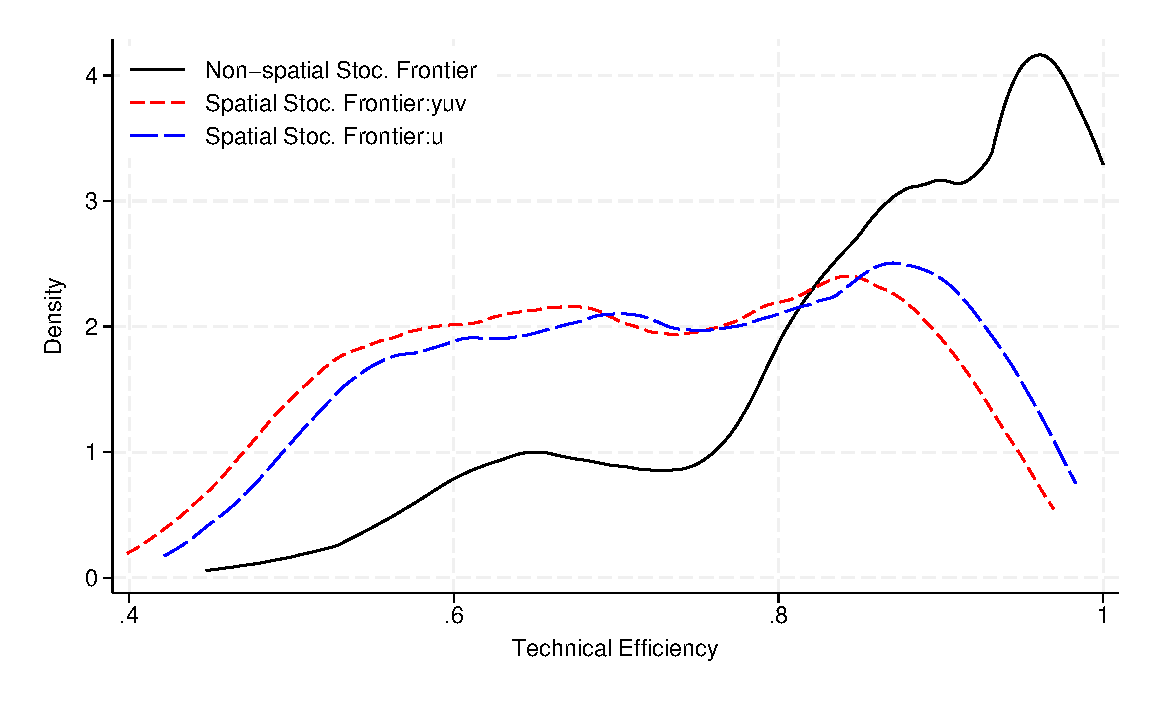
\includegraphics[height=3in]{fig1}
		\caption{Distribution of efficiency scores}
		\label{fig:fig1}
	\end{centering}
\end{figure}




 
 


\section{Conclusion}\label{sec_conclusion}
\vspace{5pt}
Geospatial units are not isolated or separated but interconnected. For instance, economic trade, social activities, and cultural exchange between different regions mutually influence each other. This spatial interdependence poses a challenge to traditional econometric methods, which generally assume cross-sectional independence. Spatial econometrics has been developed to address spatial correlation. This article presents a community-contributed command that facilitates the fitting of spatial stochastic frontier models, accounting for different sources of spatial dependence. We hope that this developed command can provide convenience to practitioners and reduce the complexity of model applications, thereby promoting robust empirical research.

However, there are certain limitations that should be acknowledged. Firstly, despite the flexibility of spatial stochastic frontier models and the introduced command, they rely on full parameterization of the spatial structure, frontier function, and distribution of random errors and inefficiency terms, following the spirit of stochastic frontier models and spatial econometrics. Model misspecification can be a potential concern, and theoretical works exploring relaxed parametric assumptions would be valuable. Secondly, as \cite{ayouba2023spatial} has recently pointed out, the spatial parametric frontier models could greatly benefit from putting identification issues and economic theory at the center of the estimation process, using e.g., the fast-growing literature on peer effects in networks. Thirdly, these models require prior information on the spatial weight matrices. Different choices of spatial weight matrices may lead to varying results. Although an  internalization of $W$ in spatial stochastic frontier models remains an open issue, \cite{ayouba2023spatial} states that Bayesian and model averaging approaches could mitigate the uncertainty arising from W. A related issue is the potencial endogeneity of the spatial weight matrix. Therefore, allowing W to be endogenous is another interesting direction of research. Finally, the numerical computation for maximum likelihood estimation (MLE) of spatial stochastic frontier models is highly complex. When dealing with large spatial weight matrices, especially when considering time-varying spatial weight matrices, the estimation process becomes computationally intensive as the matrices need to be repeatedly inverted. Additionally, the case of time-varying spatial weight matrices with large dimensions may prove memory intensive.


\section{Acknowledgments}
\vspace{5pt}
Kerui Du thanks the financial support of the National Natural Science Foundation of China (grant number 72074184). Luis Orea and Inmaculada Álvarez also thanks the financial support of the Ministry for Science and Technology  (grant number PID2020-113076GB-I00). We are grateful to Federica Galli for his Matlab codes, Federico Belotti, Silvio Daidone, Giuseppe Ilardi and Vincenzo Atella for the \stcmd{sfcross}/\stcmd{sfpanel} package, Mustafa U. Karakaplan for the \stcmd{sfkk} package, and Jan Ditzen, William Grieser and Morad Zekhnini for the \stcmd{nwxtregress} package which inspired our design of the \stcmd{xtsfsp} command. We greatly appreciate Stephen P. Jenkins (the editor) and an anonymous referee for the helpful comments and suggestions that have led to an improved version of this article and the econometric package.



\endinput



\bibliographystyle{sj}
\bibliography{sj}


\begin{aboutauthors}

Kerui Du is an associate professor at the School of Management, Xiamen University. His primary research interests include applied econometrics, energy and environmental economics.	

Luis Orea is a full professor at the School of Economics and Business, University of Oviedo. His primary research interests include Efficiency and productivity analysis, econometric modelling, agricultural economics, energy economics, regulation and competition, spatial economics. 

Inmaculada C. Álvarez is a full professor at the Department of Economics, Universidad Autónoma de Madrid. Her primary research interest include infrastructures, efficiency and productivity, economic growth and development, spatial economics and quantitative methods. 
	

	
\end{aboutauthors}


\endinput
